\section{Verklemmungen (Deadlocks)}

 \subsection{Bedingungen für das Vorliegen einer Verklemmung}
Verklemmung entsteht, wenn es einen Zyklus von Threads gibt, so dass ein Thread auf ein Betriebsmittel wartet, welches der im Zyklus nachfolgende Thread besitzt.\\
Betriebsmittel können z.B. passive Objekte sein.\\

\noindent
Folgende Bedingungen müssen erfüllt sein, damit es zu einer \textbf{Verklemmung} kommt:

\begin{enumerate}
    \item Betriebsmittel sind nur unter gegenseitigem Ausschluss nutzbar (exklusiv).
    \item Betriebsmittel, die in Verwendung sind, können dem benutzenden Thread nicht entzogen werden.
    \item Threads besitzen bereits Betriebsmittel und fordern weitere an.
    \item Folgende Bedingung gilt genau dann, wenn eine Verklemmung konkret vorliegt:
    \begin{itemize}
        \item[] Es gibt eine zyklische Kette von Threads, von denen jeder mindestens ein Betriebsmittel besitzt, das der nächste Thread in der Kette benötigt (s. Abbildung~\ref{fig:cyclic}).
        \begin{figure}
            \centering
            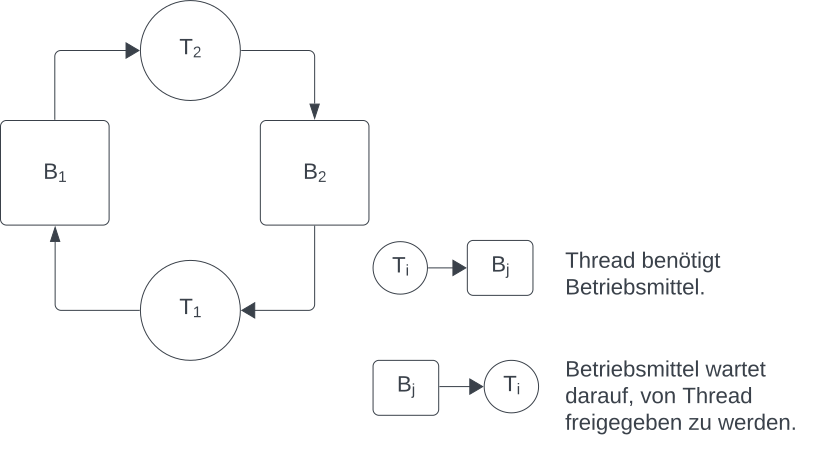
\includegraphics[scale=0.5]{chapters/fopt2/img/cyclic}
            \caption{Betriebsmittelgraph. Quelle: in Anlehnung an \cite[192, Bild 3.9]{Oec22}}
        \end{figure}
    \end{itemize}
\end{enumerate}

Vermeidung:
\begin{itemize}
    \item Anforderung ``auf einen Schlag``
    \item Anforderung in festgelegter Reihenfolge
    \item[] (Bsp.: Alle Philosophen bis auf einen fordern zuerst linke, dann rechte Gabel an.)
    \item Weitere Verfahren: Wound-Wait- und Wait-Die-Verfahren, Bankier-Algorithmus
\end{itemize}
